\documentclass[11pt,a4paper,draft]{article}
\usepackage[latin1]{inputenc}
\usepackage[margin=1in]{geometry}
\usepackage{amsmath}
\usepackage{amsfonts}
\usepackage{amssymb}
\usepackage{graphicx}
\usepackage{tikz}
\setlength\abovedisplayskip{0pt}
\author{James Brissette}
\title{CS-6350: HW 1}
\begin{document}
	\maketitle
	
	\section{Decision Trees}
	\begin{enumerate}
		\item $ $
		\begin{enumerate}
			\item $(x_1 \wedge x_2) \vee \neg x_3$   \\
				  \begin{center}
				 	\begin{tikzpicture}[grow = down, level/.style={sibling distance=60mm/#1}, node/.style = {draw, circle}]
				 	\node[node] {$x_3$}
				 	child { node[node] {1}
				 		edge from parent node [above] {0}}
				 	child { node[node] {$x_1$}
				 		child { node[node] {0}
				 			edge from parent node [above] {0}}
				 		child { node[node] {$x_2$}
				 			child { node[node] {0}
				 				edge from parent node [above] {0}}
				 			child { node[node] {1}
				 				edge from parent node [above] {1}}
				 			edge from parent node [above] {1}}
				 		edge from parent node [above] {1}};
				 	\end{tikzpicture}
				 \end{center}
			\item $x_1$ xor $(x_2 \wedge x_3)$
				\begin{center}
					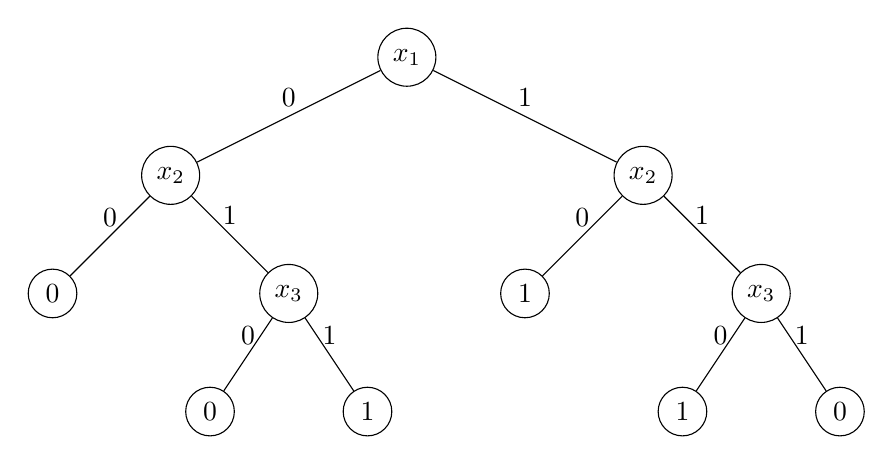
\begin{tikzpicture}[grow = down, level/.style={sibling distance=60mm/#1}, node/.style = {draw, circle}]
					\node[node] {$x_1$}
					child { node[node] {$x_2$}
						child { node[node] {0}
							edge from parent node [above] {0}}
						child { node[node] {$x_3$}
								child { node[node] {0}
									edge from parent node [above] {0}}
								child { node[node] {1}
									edge from parent node [above] {1}}
								edge from parent node [above] {1}}
						edge from parent node [above] {0}}
					child { node[node] {$x_2$}
						child { node[node] {1}
							edge from parent node [above] {0}}
						child { node[node] {$x_3$}
							child { node[node] {1}
								edge from parent node [above] {0}}
							child { node[node] {0}
								edge from parent node [above] {1}}
							edge from parent node [above] {1}}
						edge from parent node [above] {1}};
					\end{tikzpicture}
				\end{center} 
			
			\item $x_1 \wedge (x_2 \vee (x_3 \wedge x_4))$
			\begin{center}
				\begin{tikzpicture}[grow = down, level/.style={sibling distance=60mm/#1}, node/.style = {draw, circle}]
				\node[node] {$x_1$}
				child { node[node] {0}
					edge from parent node [above] {0}}
				child { node[node] {$x_2$}
					child { node[node] {$x_3$}
						child { node[node] {0}
							edge from parent node [above] {0}}
						child { node[node] {$x_4$}
							child { node[node] {0}
								edge from parent node [above] {0}}
							child { node[node] {1}
								edge from parent node [above] {1}}
							edge from parent node [above] {1}}
						edge from parent node [above] {0}}
					child { node[node] {1}
					edge from parent node [above] {1}}
				edge from parent node [above] {1}};
				
				\end{tikzpicture}
			\end{center}
		\end{enumerate}
	
		\item $ $
		\begin{enumerate}
			\item There are $2^{4}$ possible combinations of boolean inputs that each in turn generate a boolean output, and there are $2^{2^4}= 65,536$ possible boolean functions that would give every possible combination of inputs and outputs. The training dataset only provides 8 examples. As a side note, assuming a perfect data set (without noise) the training data given also eliminates the possible combinations where the same inputs would provide different outputs (e.g. \{Alphonso Red None Two\} could not produce $True$). 
			\item The entropy of the labels can be given as 
			%
			$$H(S) = -\frac{1}{2}log_{2}(\frac{1}{2}) -\frac{1}{2}log_{2}(\frac{1}{2})=1$$
			%
			\item Information Gain$_{Entropy}$ for
			%
			$$H(S_{Variety=A}) = \frac{4}{8}(1) + \frac{3}{8}(.9183) + \frac{1}{8}(0) = .8444$$
			%
			$$H(S_{Color=A}) = \frac{3}{8}(.9183) + \frac{3}{8}(.9183) + \frac{2}{8}(1) = .9387$$
			%
			$$H(S_{Smell=A}) = \frac{1}{2}(.8113) + \frac{1}{2}(.8113) = .8113$$
			%
			$$H(S_{Time=A}) = \frac{3}{8}(.9183) + \frac{5}{8}(.9710) = .9544$$
			%
			     \begin{table}[h]
			    	\centering
			    	\begin{tabular}{c|c}
			    		
			    		\hline
			    		Feature & Information Gain \\ \hline
			    		Variety & $1-.8444 = .156$ \\
			    		Color   & $1-.9387 = .061$ \\
			    		Smell   & $1-.8113 = .189$ \\
			    		Time    & $1-.9544 = .046$ \\ \hline
			    	\end{tabular}
			    	\caption{Information gain for each feature.}\label{tb-entropy-ig}
			    \end{table}
			\item Smell
			\item Decision Tree:
				\begin{center}
					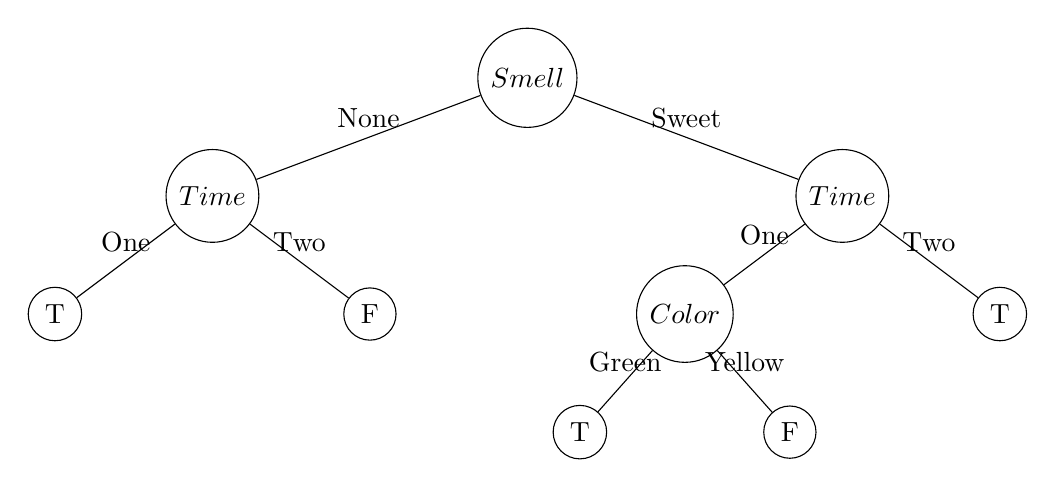
\begin{tikzpicture}[grow = down, level/.style={sibling distance=80mm/#1}, node/.style = {draw, circle}]
					\node[node] {$Smell$} % x_1
					child { node[node] {$Time$}
						child { node[node] {T}
							edge from parent node [above] {One}}
						child { node[node] {F}
							edge from parent node [above] {Two}}
						edge from parent node [above] {None}}
					child { node[node] {$Time$} % x_2
						child { node[node] {$Color$}
							child { node[node] {T}
								edge from parent node [above] {Green}}
							child { node[node] {F}
								edge from parent node [above] {Yellow}}
							edge from parent node [above] {One}}
						child { node[node] {T}
							edge from parent node [above] {Two}}
						edge from parent node [above] {Sweet}};
					\end{tikzpicture}
				\end{center}
			\item Prediction Results:
				
				\begin{table}[h!]
					\centering
					\begin{tabular}{cccc|cc}
						\hline
						Variety & Color  & Smell  & Time & Prediction & Ripe?  \\ \hline
						Alphonso& Green  & Sweet  & Two  & True  & True        \\
						Keitt   & Red    & Sweet  & One  & ?     & False       \\
						Haden   & Yellow & None   & Two  & False & True        \\ \hline
					\end{tabular}
				\end{table}
			The classifier I learned correctly predicted 1 out of the 3 new labels, incorrectly predicted another, and completely failed to account for a third (the decision tree had no way of dealing with red mangos). Dealing with a new, not before seen fruit (or one that didn't naturally fit into the decision tree) I likely would have applied the most common label, but since it's equally divided between $True$ and $False$, I would have picked $True$ for new labels (and have been wrong). Alternatively, I may have chosen to pick the most frequent label for the new item not represented in the table (red mangos), which was also $True$ and equally as wrong. My accuracy was 
			%
			$$1 for 3 = \frac{1}{3} = .333$$
			%.
		\end{enumerate}
	
		\item $ $
		\begin{enumerate}
			\item Information Gain using Majority Error can be thought of in the same way:
			%
			$$InformationGain_{ME}(S_{A}) = ME(S) - ME(S_A)$$ where $S$ is your training data and $A \in Attribute Space$ is the attribute being split on. The difference between the two represents the decrease in your error (based on the training data) of splitting on attribute $A$. $ME(S_A)$ is the sum of the MajorityErrors for each possibility under $A$ and is weighted by the relative probabilities of the attribute taking on each possible value of $A$ (apologies if the below isn't correct notation, I simply wanted to try and express the idea mathematically):
			\\
			$$ME(S_{A}) = \sum_{a \in A}^{}p_{A=a}*ME(S_{A=a})$$
			%
			\item Values were calculated separately (not all work is shown here). Additionally, the below were calculated using only the training examples from the original table as the text did not explicitly state to include the additional three examples from question 2f in subsequent calculations. $ME(S)$ can be given as follows:
			%
			$$ME(S) = 1 - \max\limits_{T,F}(T=\frac{1}{2},F=\frac{1}{2}) = 1 - \frac{1}{2}= \frac{1}{2}$$
			%
			Example Calculation for Variety:
			$$ME(S_{Variety=Alphonso}) = 1 - \max\limits_{alphonso}(T=\frac{1}{2},F=\frac{1}{2}) = 1 - \frac{1}{2}= \frac{1}{2}$$
			%
			$$ME(S_{Variety=Keitt}) = 1 - \max\limits_{keitt}(T=\frac{1}{3},F=\frac{2}{3}) = 1 - \frac{2}{3}= \frac{1}{3}$$
			%
			$$ME(S_{Variety=Haden}) = 1 - \max\limits_{haden}(T=1,F=0) = 1 - 1= 0$$
			%
			And Information Gain using MajorityError and splitting on variety gives:
			$$IG_{ME}(S_{A=Variety}) = ME(S) - \sum_{a \in A}p_{A=a}*ME(S_{A=a}) = \frac{1}{2} - \frac{1}{2}(\frac{1}{2}) - \frac{3}{8}(\frac{1}{3}) - \frac{1}{8}(0)$$ $$=\frac{1}{8}$$
				 \begin{table}[h!]
					\centering
					\begin{tabular}{c|c}
						\hline
						Feature & Information Gain (using majority error) \\ \hline
						Variety &       .125        \\
						Color   &       .125         \\
						Smell   &       .250          \\
						Time    &       .133           \\ \hline
					\end{tabular}
					\caption{Information gain for each feature.}\label{tb-maj-ig}
				\end{table}
			%
			
			\item According to ID3 using ME as an estimate for the "best" feature to split on, "Smell" still yields the largest information gain. However, Entropy and MajorityError ranked the features differently based on information gain, and I would venture to say that even though "Smell" was the root of both trees, this does not necessarily mean that they would create the same tree if run to completion.
		\end{enumerate}	
	\end{enumerate}
	
	\section{Linear Classifier}
		\begin{enumerate}
			\item A linear classifier compatible with the given data set is given by the below:
			\begin{center}
				$w_1=0$, $w_2=0$, $w_3=1$, $w_4=1$, $b=0$
			\end{center}
		
			\item My classifier actually performed pretty poorly when tested on the extended data set:\\
				$$\begin{array}{cccc|c|c}
					x1 & x2 & x3 & x4 & Prediction & o \\ \hline
					0 & 0 & 0 & 0 & -1 & -1 \\
					0 & 0 & 0 & 1 & 1  & -1 \\
					0 & 0 & 1 & 0 & 1  & -1 \\
					0 & 0 & 1 & 1 & 1  & -1 \\
					1 & 0 & 1 & 1 & 1  & 1  \\
					1 & 1 & 0 & 1 & 1  & 1
				\end{array}$$ It correctly predicted 3 out of the 6 additional items, or a success rate of $0.5$.
				
				\item The correct linear classifier for the complete set is:
				\begin{center}
					$w_1=\frac{1}{3}$, $w_2=\frac{1}{3}$, $w_3=\frac{1}{3}$, $w_4=\frac{1}{3}$, $b=-1$
				\end{center}
			
		\end{enumerate}
	
	\section{Experiments}
		\begin{enumerate}
			\item $ $
			\begin{enumerate}
				\item For this problem I thought it best to first implement both functions for information gain (e.g.\textbf{ findEntropy()} and \textbf{findMajorityErr(})) so as to have a measurement from which to assess the "best" element to split on when it came time to implement ID3. After that I defined a Node class that knew its own label, its parent, and it's children. This allowed me to utilize the provided code and begin to build the heirarchy needed and ultimately develop the tree structure.
				
				Then I implemented the ID3 algorithm per the lecture slides and was left with a single root node who knew its children, and all of its children who knew their parent and their each of their respective children. The data input for this funtion was the Data.data type (not the np.ndarray type) which allowed for the use of the unique Data.data functions to query specific columns and attributes. For ease of implementation, I assigned each unique possible value of the root to its child attribute, which essential made the children attribute of the root more like its branches. Each of its branches' children were the next nodes down in what one would visually determine were the roots actual children.
				
				 The next step was to define a tree class that was able to perform meaningful operations on the nodes, and I implemented a Tree class with methods that allowed the tree to calculate its depth and predict the labels for new data that could be passed to it. The prediction ultimately converted the input to a ndarray I also added a few additional methods and functions that I used to integrate this assignment with the Visualization for Data Science homework that allowed me to render the tree in a web browser. Lastly, I wrote a \textbf{crossValidate(fold)} function that takes fold as an integer and performs the cross-validation process reporting the accuracy of the tree on the training data.
				 
				 \item My tree reported an accuracy of $100\%$ for the training data in \textbf{data/train.csv}
				 
				 \item I was a little surprised but my tree also reported an accuracy of $100\%$ on the test data in \textbf{data/test.csv}.
				 
				 \item The maximum depth of my decision tree was \textbf{6 nodes}.
				
			\end{enumerate}
		
			\item $ $
			\begin{enumerate}
				\item $$
				\begin{array}{c|cc}
					Depth & Avg. Validation Accuracy & Std. Dev \\ \hline
					1  & 0.77411945  & 0.20390952   \\
					2  & 0.92633997  & 0.07951074   \\
					3  & 0.95313936  & 0.02693425   \\
					4  & 0.95987749  & 0.02993316   \\
					5  & 0.96692190  & 0.03234251   \\
					10 & 0.96906585  & 0.03417651   \\
					15 & 0.96906585  & 0.03417651   \\
				\end{array}
				$$ A depth of 10 should be chosen as the best given the information in the table above. The average validation accuracy of that depth is the greatest, and since we are cross validating, we can take this to mean the predicted accuracy of the tree on the test set is likely to be the highest as well. The standard deviation of the that depth is slightly higher than a depth of 5, however, it also has a higher average, so I believe that is of little consequence in this case.
				
				\item Re-running the now cross-validated decision tree with a depth of \textbf{10} on the \\\textbf{data/test.csv} file, I am happy to announce my tree reported an accuracy of $100\%$.
				
				\item In this particular case I think it is difficult to say. It seems as though the dataset was such that the training data perfectly predicted the test data, and so in this instance there was no notable difference between the depth-limited tree capped at 10 nodes and the full decision tree with a max depth of 6 nodes. However, it's important to keep in mind that rarely will we ever get so clean and complete data as this, and with so little noise. The depth limited tree is an excellent way to combat over-fitting our training model to the data and ultimately making poor predictions. I do think limiting depth is a good idea, and I think given another data set, its advantages would be more pronounced and evident.
			\end{enumerate}
		\end{enumerate}
	
\end{document}